\chapter{Background}
\label{chapter2}
In this chapter, we discuss the background knowledge and introduce notation that will be used for the thesis. We begin with intruding graphical models formally, which is followed with the inference tasks of graphical models. We also discusses the learning principles in model learning. \textcolor{blue}{Provide more thorough explanation here after this chapter is finished}.

\section{Graphical Models}
Graphical models provide a formal graph representation of statistical dependency of complex problems. The conditional independence of any random variables can be conveniently analyzed in a graphical model (I-map, d-Separation, markov blanket[]). More importantly, a intractable complex problem can be resolved by local interactions of small parts of a graphical model.

More formally, a graphical model is a representation of a collection of random variables (along their domains) and nonnegative functions. Let $\bm{X}= (X_1, X_2, \cdots, X_N)$ be a vector of random variables, where an element variable $X_i$ can be either discrete or continuous and takes values from its domain $\Xx_i$. Note that domain of a random variable is not necessary be the same as that of another.

We use lower case letters, e.g. $x_i \in \Xx_i$, to indicate a value assignment of $X_i$. Similarly, $\bm{x}$ denotes the assignment of $\bm{X}$, and
\begin{equation}
  p(x_1, x_2, \cdots, x_N) = P(X_1 = x_1, X_2 = x_2, \cdots, X_N = x_N),
\end{equation}
which sometimes is simplified as $p(\bm{x})=P(\bm{X}=\bm{x})$.

A graphical model over random variable $\bm{X}$ consists of a set of local nonnegation functions. In directed graphical models, i.e. Bayesian networks, the local functions are conditional probability function. The joint probability distribution is represented as product of these conditional probability functions, i.e. $p(\bm{x}) = \prod_{n=1}^{N}p(x_n| \Pp(x_n))$ where $\Pp(\cdot)$ denotes the set of parent nodes in the directed graph. A Bayesian network is usually easier to be interpreted due to the fact that the its local functions are conditional probabilities. But Bayesian networks can only to applied to limited cases where influence between variables is directional. In many practical cases, interaction between variables can not be naturally described by impact with directionality. Problems of this kind can be represented by undirected graphical models, i.e. Markov random field (MRF). Under certain condition, a Bayesian network can be perfectly represented by a Markov random field without loss of independence information by moralizing edges \cite[Chapter~4.5]{koller2009pgm}. Instead of conditional probability, the local functions of MRF represents the compatibility of states of different variables, which are known as potential factors in literature. Different from conditional probabilities the Bayesian network, the potential factors in MRFs are not necessary summed to one. We provide a toy example of MRF with three variable nodes as follows.
\begin{figure}[!t]
  % \captionsetup[subfigure]{justification=centering}
  \begin{subfigure}{.3\textwidth}
    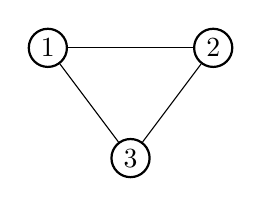
\begin{tikzpicture}
      \begin{scope}[scale=0.7]
        \tikzstyle{cnode} = [thick, draw=black, circle, inner sep = 2pt,  align=center]
        \node[cnode] (x1) at (0,0) {$1$};
        \node[cnode] (x2) at (3,0) {$2$};
        \node[cnode] (x3) at (1.5,-2) {$3$};
        \draw[-] (x1) -- (x2);
        \draw[-] (x1) -- (x3);
        \draw[-] (x2) -- (x3);
      \end{scope}
    \end{tikzpicture}
  \end{subfigure}
  \begin{subfigure}{0.3\textwidth}
    \begin{tabular}{llc}
      \toprule
      $X_1$ & $X_2$ & $\phi(X_1, X_2)$ \\
      \midrule
      0  &  0  &  10 \\
      0  &  1  &  1 \\
      1  &  0  &  1 \\
      1  &  1  &  10\\
      \bottomrule
    \end{tabular}
  \end{subfigure}
  \begin{subfigure}{0.05\textwidth}
    \centering
    \begin{tikzpicture}
      \node[] at (0,0) {$\cdots$};
    \end{tikzpicture}
  \end{subfigure}
  \begin{subfigure}{0.3\textwidth}
    \begin{tabular}{llc}
      \toprule
      $X_2$ & $X_3$ & $\phi(X_1, X_2)$ \\
      \midrule
      0  &  0  &  5 \\
      0  &  1  &  3 \\
      1  &  0  &  3 \\
      1  &  1  &  5 \\
      \bottomrule
    \end{tabular}
  \end{subfigure}
  \caption{A Markov random field with three binary nodes. Potential factors are represented by tables.}
  \label{chp2:tab:toy_mrf}
  \hspace{1cm}
\end{figure}

\begin{example}\label{chpt2:mrf-3node-example}
  As shown in Figure~\ref{chp2:tab:toy_mrf}, the MRF encodes dependency of three random variables $X_1$, $X_2$, and $X_3$, where node $i$ is associated with variable $X_i$ and each has a binary domain, i.e. $\Xx_i = {0,1}$ for $i =1,2,3$. Three potential factors of the MRF together define the joint distribution
  \begin{equation*}
    p(\bm{x}) = \frac{1}{Z} \phi_{1,2}(x_1, x_2) \phi_{2,3}(x_2, x_3) \phi_{1,3}(x_1, x_3)
  \end{equation*}
  where $Z = \sum_{x_1, x_2, x_3}\phi_{1,2}(x_1, x_2) \phi_{2,3}(x_2, x_3) \phi_{1,3}(x_1, x_3)$ normalizes the potential factors such that $p(\bm{x})$ sums to one. The exemplified potential factors in Figure~\ref{chp2:tab:toy_mrf} demonstrate that it is more compatible or likely when $X_1$, $X_2$ and $X_3$ are in the same state (either $0$ or $1$) than they are configured into different states.
\end{example}

From the above example to a formal statement, a MRF over random vector $\bm{X}$ can be represented by a undirected graph $\Gg(\Vv, \Ee)$, with each node $i \in \Vv$ is associated with a random variable $X_i$ and undirected edge set $\Ee \subset \Vv \times \Vv$. This MRF encodes a collection of distributions that factorize as
\begin{equation}\label{chp2:eq:mrf-definition}
  p(\bm{x};\bm{\theta}) = \frac{1}{Z(\bm{\theta})} \prod_{\alpha \in \Ii} \phi_{\alpha}(\bm{x_{\alpha}};\bm{\theta}),
\end{equation}
where $\Ii$ is the set of indexes of potential factors, and each factor $\phi_{\alpha}$ for $\alpha\in \Ii$ is defined on subset of $\bm{X}$, i.e. $\phi_{\alpha}: \Xx_{\alpha} \rightarrow \RR^{+} \cup \{0\}$, where $\Xx_{\alpha} = \prod_{i\in \alpha}\Xx_i$ is the domain of potential factor $\phi_{\alpha}$. The scope of factor $\alpha$ is $\bm{X}_{\alpha} = \left\{ X_i| i\in \alpha \right\}$. In \eqref{chp2:eq:mrf-definition},
\begin{equation}
  Z(\bm{\theta}) = \sum_{\bm{x}} \prod_{\alpha \in \Ii} \phi_{\alpha}(\bm{x_{\alpha}};\bm{\theta})
\end{equation}
is the \textit{partition function}. Apparently, the partition function normalizes the potential factors such that $p(\bm{x}; \bm{\theta})$ is a proper probability.


We would focus mainly on the undirected graphical models here.


It is clear that undirected graphs should be explained, since Part I is work on it. For HMM, it can be viewed either a dynamic Bayesian network (chapter 6, Koller) or condition random field(introduction to CRF, Sutton).


\subsection{Alternative Representation of MRF}
\begin{figure}[!t]
  % \captionsetup[subfigure]{justification=centering}
  \begin{subfigure}{.5\textwidth}
    \centering
    \begin{tikzpicture}
      \begin{scope}[scale=0.7]
        \tikzstyle{cnode} = [thick, draw=black, circle, inner sep = 2pt,  align=center]
        \tikzstyle{nnode} = [thick, rectangle, rounded corners = 0pt,draw,inner sep = 5pt]
        \node[cnode] (x1) at (0,0) {$1$};
        \node[above=0.2mm of x1] {$X_1$};
        \node[cnode] (x2) at (3,0) {$2$};
        \node[above=0.2mm of x2] {$X_2$};
        \node[cnode] (x3) at (1.5,-2) {$3$};
        \node[below=0.2mm of x3] {$X_3$};

        \node[nnode] (f12) at (1.5, 0) {};
        \node[] at ($(f12) + (0,0.6)$) {$\phi_{1,2}$};
        \node[nnode] (f13) at (0.75, -1) {};
        \node[] at ($(f13) + (-0.8,0)$) {$\phi_{1,3}$};
        \node[nnode] (f23) at (2.25, -1) {};
        \node[] at ($(f23) + (0.80,0)$) {$\phi_{2,3}$};
        \path[-, draw, thick]
        (x1) edge node {} (f12)
        (f12) edge node {} (x2)
        (x2) edge node {} (f23)
        (f23) edge node {} (x3)
        (x3) edge node {} (f13)
        (f13) edge node {} (x1)
        ;
      \end{scope}
      
    \end{tikzpicture}
    \caption{Factor graph of Example~\ref{chpt2:mrf-3node-example}}
  \end{subfigure}
  \begin{subfigure}{.5\textwidth}
    \centering
    \begin{tikzpicture}
      \begin{scope}[scale=0.7]
        \tikzstyle{cnode} = [thick, draw=black, circle, inner sep = 2pt,  align=center]
        \tikzstyle{cfnode} = [thick, draw=black, fill=gray,circle, inner sep = 2pt,  align=center]
        \tikzstyle{nnode} = [thick, rectangle, rounded corners = 0pt,draw,inner sep = 5pt]
        \node[cnode] (x1) at (0,0) {$1$};
        \node[above=0.2mm of x1] {$X_1$};
        \node[cfnode] (x2) at (3,0) {$2$};
        \node[above right=0.2mm and 0.2mm of x2] {$X_2=x_2$};
        \node[cnode] (x3) at (1.5,-2) {$3$};
        \node[below=0.2mm of x3] {$X_3$};
        \node[nnode] (f12) at (1.5, 0) {};
        \node[] at ($(f12) + (0.2,0.6)$) {$\phi_{1,2}\bm{1}(x_2)$};
        \node[nnode] (f13) at (0.75, -1) {};
        \node[] at ($(f13) + (-0.8,0)$) {$\phi_{1,3}$};
        \node[nnode] (f23) at (2.25, -1) {};
        \node[] at ($(f23) + (1.50,0)$) {$\phi_{2,3}\bm{1}(x_2)$};
        \path[-, draw, thick]
        (x1) edge node {} (f12)
        (f12) edge node {} (x2)
        (x2) edge node {} (f23)
        (f23) edge node {} (x3)
        (x3) edge node {} (f13)
        (f13) edge node {} (x1)
        ;
      \end{scope}
    \end{tikzpicture}
    \caption{Conditioning on $X_2=x_2$}
  \end{subfigure}

  \caption{A Markov random field with three binary nodes. Potential factors are represented by tables.}
  \label{chp2:tab:toy-factor-graph}
  \hspace{1cm}
\end{figure}

The representation of a MRF by $\Gg(\Vv, \Ee)$ as explained above is compact, but the potential factors are missing. An alternative representation of MRF is \textit{factor graph}\cite{}, which is a bipartite graph topology. In a factor graph, a potential factor is explicitly represented as a factor node, as counterpart of variable node associated with a random variable.
\begin{definition}\label{chpt2:def:factor-graph}
  A factor graph $\Gg_F$, is a bipartite graph that represents the factorization structure of \eqref{chp2:eq:mrf-definition}. A factor graph has two types of nodes: i) a variable node for each variable $x_i$; ii) a factor node for each potential function $\phi_{\alpha}$. An edge between a variable node $i$ and factor node $\alpha$ if and only if $x_i$ is argument of $\phi_{\alpha}$. We would denote a factor graph by $\Gg_F(\Vv \cup \Ff, \Ee_F)$ with $\Vv$ as the set of variable nodes, $\Ff$ as the set of factor nodes, and $\Ee_F$ the set of undirected edges.
\end{definition}
\begin{example}
  factor graph of example \ref{chpt2:mrf-3node-example}.
\end{example}


\subsection{Conditioning on Observations}
It is not rare that a graphical model may contain observed variable. The node set of a MRF can be separated into a subset $\Vv_O$ of nodes, that are associated with observed variable $\bm{X}_O$, and a subset $\Vv_U$ of nodes associated with unobserved variable $\bm{X}_U$. For an observation $\bm{X}_O=\bm{x}_o$,
\begin{equation}
  p(\bm{x}_u|\bm{x}_o;\bm{\theta}) = \frac{p(\bm{x}; \bm{\theta})}{p(\bm{y};\bm{\theta})} =  \frac{Z(\bm{y},\bm{\theta})}{Z(\bm{\theta})},
\end{equation}
where 
\begin{align}
  \tilde{p}(\bm{x}; \bm{\theta}) &= \prod_{\alpha \in \Ii} \phi_{\alpha}(\bm{x_{\alpha}};\bm{\theta}), \nonumber \\
  Z(\bm{x}_o, \bm{\theta}) &= \sum_{\bm{x}_u} \tilde{p}(\bm{x}; \bm{\theta}), \nonumber \\
  Z(\bm{\theta}) &= \sum_{\bm{x}_o}\sum_{\bm{x}_u} \tilde{p}(\bm{x}; \bm{\theta}).
\end{align}
This means that a condition probability can be computed by partition function and sub-partition functions. Alternatively, the conditional probability can be written as
\begin{equation}
  p(\bm{x}_u|\bm{x}_o;\bm{\theta}) = \frac{\tilde{p}(\bm{x}; \bm{\theta})\bm{1}(\bm{x}_o)}{\sum_{\bm{x}_u}\tilde{p}(\bm{x}; \bm{\theta})\bm{1}(\bm{x}_o)}
\end{equation}
where $\bm{1}(\bm{x}_o)$ is an indicator function and equals to one if and only if the states of nodes in $\Vv_o$ are jointly $\bm{x}_o$. This can be understood as clamping nodes in $\Vv_o$ of the MRF to configuration $\bm{x}_o$, i.e. the domain of $\bm{X}_O$ becomes a set containing only $\bm{x}_o$. Then any inference applicable to a MRF applies to the MRF with nodes clamped as well.

In addition to the above intuitions, conditioning can also be understood as a process of reducing the graph of a MRF. When a MRF is conditioned on $\bm{x}_o$, the variables nodes of set $\Vv_O$ are removed from $\Gg$, along with their edges. The potential factors with regarding to $\Vv_U$ are modified accordingly \cite[Chapter~4.2.3]{koller2009pgm}.

It can be seen that MRF framework is capable to handle conditioning as well. Therefore, in the following part of the thesis, it might or might not have bee based on conditioning observed variables when a MRF is mentioned.

\section{Inference Tasks}
\label{sec:background-graphial-reppresentation}
refer to 2.3 of Domke TPAMI and 2.3 of Wainwright graphical models.

\subsection{intro to inference methods}
\section{Learning principles}
\subsection{Learning of Full Observation}

the learning diagram here
\begin{itemize}
\item Structural learning
\item parameter learning
\end{itemize}


the learning principle:
\begin{itemize}
\item Maximal likelihood estimation (MLE)
\item Bayesian estimation
\item Maximal conditional likelihood
\item Maximal '' `Margin`''
\item Maximum entropy
\end{itemize}


It may be better to discuss the learning principle here.

Cited from 10-708 lecture6 note:

UNOBSERVED VARIABLES:

A variable can be unobserved or latent because it is a(n):

-Abstract or imaginary quantity meant to simplifiy the data generation process, e.g. speech recognition models, mixture models.
-A real-world object that is difficult or impossible to measure, e.g. the temperature of a star, causes of disease, evolutionary ancestors.
-A real-world object that was not measured due to missed samples, e.g. faulty sensors.

Discrete latent variables can used to partition or cluster data into sub-groups

Continuous latent variables (factors) can be used for dimensionality reduction (e.g. factor analysis, etc)
\subsection{Dealing with latent variables}
\subsection{about clamping node}
clamping node gives conditional distribution.

\subsection{about ELBO bound}
1. the bound used by EM

2. talk about ELBO/variational inference \href{https://media.nips.cc/Conferences/2016/Slides/6199-Slides.pdf}{Variational Inference}, which is closely related the bound used in EM.

%%% Local Variables:
%%% mode: latex
%%% TeX-master: "../../main"
%%% End:
